\documentclass{article}
\usepackage[utf8]{inputenc}
\usepackage{amsmath}
\usepackage{amssymb}
\usepackage{graphicx}
\usepackage{hyperref}
\usepackage{tikz}
\usepackage{pgfplots}
\usepackage{float}
\usepackage{listings}
\usepackage{color}
\usepackage{bbm}
\usepackage{multirow}
\usepackage{comment}

\newcommand{\wb}{\mathbf{w}}
\newcommand{\xb}{\mathbf{x}}

\title{Reinforcement Learning \\ Exercise 8 - Solution}
\author{Jonathan Schnitzler - st166934 \\
Eric Choquet - st160996}
\date{\today}
\begin{document}
\maketitle

\section{n-step TD compared to planing}

\paragraph*{a) Improve TD(0) with n-step TD}
The difference of the n-step temporal difference to the Dyna-Q planning, is that only the reward of the path which was taken can be accounted for. Therefore, unlike the image it is not possible after one episode to have a policy for all tiles, but instead only for the taken path. In contrast, Dyna-Q planning revisits arbitrary a virtual tile, which allows a richer interpretation. A visual interpretation is depicted in Figure \ref{fig:1a}.

\begin{figure}[H]
\centering
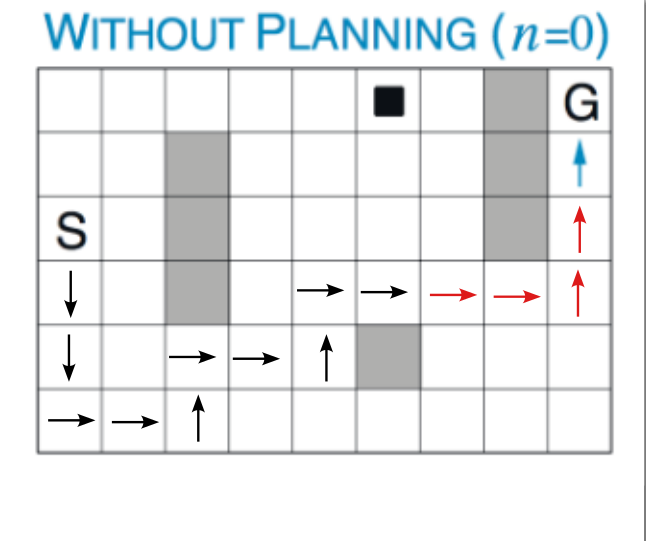
\includegraphics[width=0.5\textwidth]{nstep.png}
\caption{The red arrows indicate 4-step TD, while the black arrows just continue for an arbitrary n, where the sampled episode is also arbitrary}
\label{fig:a1}
\end{figure}

\paragraph*{b) Recursive lambda-return}

The $\lambda$-return is defined as
\begin{equation}
    G_{t}^{\lambda} = (1-\lambda)\sum_{n=1}^{\infty}\lambda^{n-1}G_{t:t+n}
\end{equation}
with
\begin{equation}
    G_{t:t+n} = R_{t+1} + \gamma R_{t+2} + \ldots + \gamma^{n-1}R_{t+n} + \gamma^{n}V(S_{t+n})
\end{equation}
To define it recursively, we want to reframe the problem involving $G_t^{\lambda}$
\begin{equation}
    G_{t+1}^{\lambda} = (1-\lambda)\sum_{n=1}^{\infty}\lambda^{n-1}G_{t+1:t+n+1}
\end{equation}
Here we can note that
\begin{equation}
    G_{t+1:t+n+1} = R_{t+2} + \gamma R_{t+3} + \ldots + \gamma^{n-1}R_{t+n+1} + \gamma^{n}V(S_{t+n+1})
\end{equation}
We can rewrite $G_{t+1:t+n+1}$ as
\begin{equation}
    G_{t+1:t+n+1} = \frac{1}{\gamma}\left(G_{t:t+n} - R_{t+1} + \gamma^{n} R_{t+n+1} -\gamma^n V(S_{t+n})\right)+ \gamma^{n}V(S_{t+n+1})
\end{equation}

Then we can rewrite the $\lambda$-return as

\begin{align*}
    G_{t+1}^{\lambda} &= (1-\lambda)\sum_{n=1}^{\infty}\lambda^{n-1} \left[ \frac{1}{\gamma}\left(G_{t:t+n} - R_{t+1} + \gamma^{n} R_{t+n+1} -\gamma^n V(S_{t+n})\right) + \gamma^{n}V(S_{t+n+1}) \right] \\
    G_{t+1}^{\lambda} &= \frac{1}{\gamma}(1-\lambda)\sum_{n=1}^{\infty}\lambda^{n-1}G_{t:t+n}
    \\ &+ (1-\lambda)\sum_{n=1}^{\infty}\lambda^{n-1} \left[ \frac{1}{\gamma}\left(- R_{t+1} + \gamma^{n} R_{t+n+1} -\gamma^n V(S_{t+n})\right) + \gamma^{n}V(S_{t+n+1}) \right] \\
    G_{t+1}^{\lambda} &= \frac{1}{\gamma} G_t^{\lambda}+ (1-\lambda)\sum_{n=1}^{\infty}\lambda^{n-1} \left[ -\frac{R_{t+1}}{\gamma} + \gamma^{n-1} R_{t+n+1} -\gamma^{n-1} V(S_{t+n}) + \gamma^{n}V(S_{t+n+1}) \right]
\end{align*}

Could be extended further, but this should be sufficient for today.

% https://ai.stackexchange.com/questions/11783/how-can-the-lambda-return-be-defined-recursively is different

\section{n-step Sarsa on the Frozen Lake}

The implemented algorithm in python with the Gym FrozenLake Environment can be found attached to this file. The 8x8 map is the following
\begin{table}[H]
\centering
\begin{tabular}{ccccccccc}
S&F&F&F&F&F&F&F\\
F&F&F&F&F&F&F&F\\
F&F&F&H&F&F&F&F\\
F&F&F&F&F&H&F&F\\
F&F&F&H&F&F&F&F\\
F&H&H&F&F&F&H&F\\
F&H&F&F&H&F&H&F\\
F&F&F&H&F&F&F&G
\end{tabular}
\caption{Where F is frozen, H is hole, S is start and G is goal}
\label{tab:map}
\end{table}

The value function after 250000 episodes with $\alpha = 0.025$ and $\epsilon = 0.1$ is depicted in Figure \ref{fig:V} and the state-action value function in Figure \ref{fig:Q}. The policy is given in Table \ref{tab:policy}.

\begin{figure}[H]
\centering
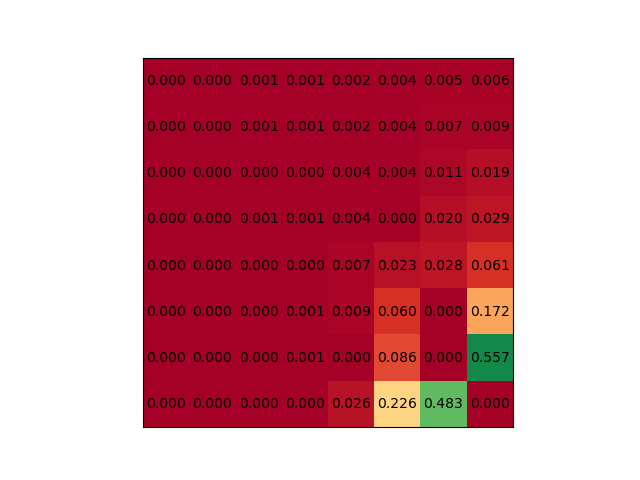
\includegraphics[width=0.8\textwidth]{images/V.png}
\caption{Value function after 250000 episodes}      
\label{fig:V}
\end{figure}

\begin{figure}[H]
\centering
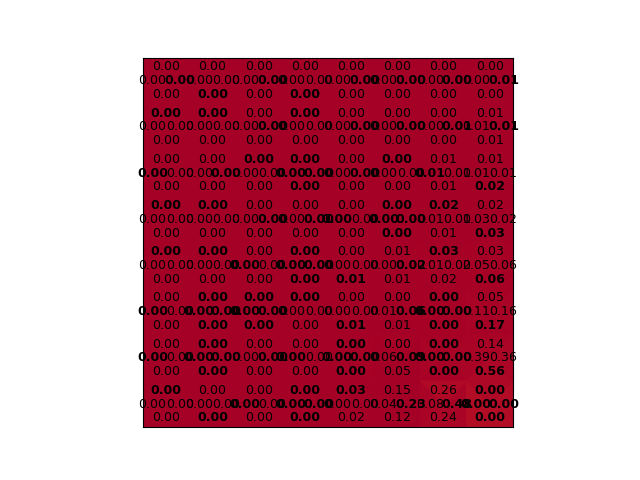
\includegraphics[width=0.8\textwidth]{images/Q.png}
\caption{State-Action value function after 250000 episodes}
\label{fig:Q}
\end{figure}

\begin{figure}[H]
\centering
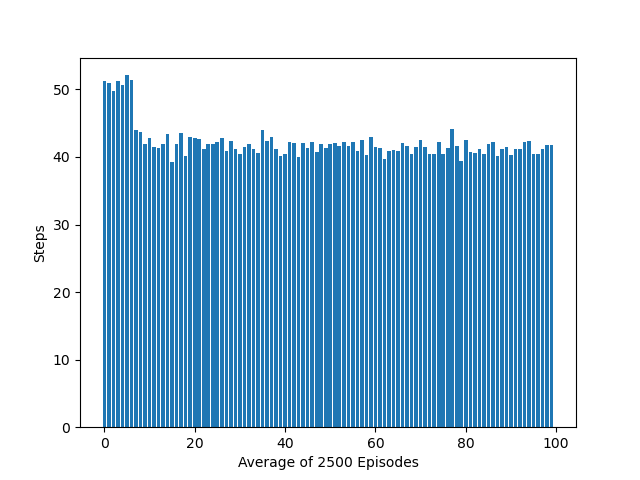
\includegraphics[width=0.8\textwidth]{images/avg_episode_length.png}
\caption{Average episode length through the training process}
\label{fig:avg}
\end{figure}

\begin{table}[H]
    \centering
    \begin{tabular}{ccccccccc}
        →& ↓& →& ↓& →& →& →& → \\
        ↑& ↑& →& ↑& →& →& →& → \\
        ←& →& ↑& H& →& ↑& ←& ↓ \\
        ↑& ↑& →& →& ←& H& ↑& ↓ \\
        ↑& ↑& ←& H& ↓& →& ↑& ↓ \\
        ←& H& H& ↑& ↓& →& H& ↓ \\
        ←& H& →& ←& H& →& H& ↓ \\
        ↑& ↓& ←& H& ↑& →& →& G 
    \end{tabular}
\caption{Where the arrow indicates the walking direction}
\label{tab:policy}
\end{table}


\end{document}
